
% Model Results

% Table created by stargazer v.5.2.2 by Marek Hlavac, Harvard University. E-mail: hlavac at fas.harvard.edu
% Date and time: Sun, Dec 16, 2018 - 10:46:24 AM
\begin{table}[!htbp] \centering 
  \caption{} 
  \label{} 
\begin{tabular}{@{\extracolsep{5pt}}lccc} 
\\[-1.8ex]\hline 
\hline \\[-1.8ex] 
 & \multicolumn{3}{c}{\textit{Dependent variable:}} \\ 
\cline{2-4} 
\\[-1.8ex] & \multicolumn{3}{c}{isCorrect} \\ 
\\[-1.8ex] & (1) & (2) & (3)\\ 
\hline \\[-1.8ex] 
 baselineHazardRate & 0.747 & 2.292$^{*}$ & $-$0.717 \\ 
  & (0.485) & (1.390) & (3.685) \\ 
  & & & \\ 
 baselineHazardRate2 &  & $-$7.775$^{***}$ & $-$41.398$^{**}$ \\ 
  &  & (2.587) & (18.429) \\ 
  & & & \\ 
 baselineHazardRate3 &  &  & 72.938$^{***}$ \\ 
  &  &  & (24.482) \\ 
  & & & \\ 
 treatmentHazardRatio & $-$2.489$^{***}$ & 0.177 & $-$5.440$^{**}$ \\ 
  & (0.181) & (0.744) & (2.463) \\ 
  & & & \\ 
 treatmentHazardRatio2 &  & $-$3.610$^{***}$ & 12.625$^{**}$ \\ 
  &  & (0.785) & (6.059) \\ 
  & & & \\ 
 treatmentHazardRatio3 &  &  & $-$12.838$^{***}$ \\ 
  &  &  & (4.145) \\ 
  & & & \\ 
 cohortSize & 0.031$^{***}$ & 0.074$^{***}$ & 0.169 \\ 
  & (0.005) & (0.023) & (0.116) \\ 
  & & & \\ 
 cohortSize2 &  & $-$0.001 & $-$0.004 \\ 
  &  & (0.001) & (0.008) \\ 
  & & & \\ 
 cohortSize3 &  &  & 0.00003 \\ 
  &  &  & (0.0002) \\ 
  & & & \\ 
 expectedLifetimes & 0.015$^{***}$ & 0.092$^{***}$ & 0.527$^{***}$ \\ 
  & (0.005) & (0.018) & (0.051) \\ 
  & & & \\ 
 expectedLifetimes2 &  & $-$0.001$^{***}$ & $-$0.020$^{***}$ \\ 
  &  & (0.0002) & (0.002) \\ 
  & & & \\ 
 expectedLifetimes3 &  &  & 0.0002$^{***}$ \\ 
  &  &  & (0.00002) \\ 
  & & & \\ 
 pctOpenEnrollmentPeriods & 0.144 & 5.700$^{***}$ & 3.995 \\ 
  & (0.137) & (0.760) & (2.697) \\ 
  & & & \\ 
 pctOpenEnrollmentPeriods2 &  & $-$4.431$^{***}$ & 0.517 \\ 
  &  & (0.633) & (6.656) \\ 
  & & & \\ 
 pctOpenEnrollmentPeriods3 &  &  & $-$2.858 \\ 
  &  &  & (4.275) \\ 
  & & & \\ 
 Constant & 0.599$^{***}$ & $-$1.233$^{***}$ & $-$1.835$^{***}$ \\ 
  & (0.128) & (0.261) & (0.544) \\ 
  & & & \\ 
\hline \\[-1.8ex] 
Observations & 2,098 & 2,098 & 2,098 \\ 
Log Likelihood & $-$1,323.611 & $-$1,276.167 & $-$1,209.716 \\ 
Akaike Inf. Crit. & 2,659.222 & 2,574.334 & 2,451.432 \\ 
\hline 
\hline \\[-1.8ex] 
\textit{Note:}  & \multicolumn{3}{r}{$^{*}$p$<$0.1; $^{**}$p$<$0.05; $^{***}$p$<$0.01} \\ 
\end{tabular} 
\end{table}  

% Table created by stargazer v.5.2.2 by Marek Hlavac, Harvard University. E-mail: hlavac at fas.harvard.edu
% Date and time: Sun, Dec 16, 2018 - 5:03:42 PM
\begin{table}[!htbp] \centering 
  \caption{} 
  \label{} 
\begin{tabular}{@{\extracolsep{5pt}}lccc} 
\\[-1.8ex]\hline 
\hline \\[-1.8ex] 
 & \multicolumn{3}{c}{\textit{Dependent variable:}} \\ 
\cline{2-4} 
\\[-1.8ex] & \multicolumn{3}{c}{isCorrect} \\ 
\\[-1.8ex] & (1) & (2) & (3)\\ 
\hline \\[-1.8ex] 
 baselineHazardRate & 1.340$^{***}$ & 0.751 & $-$2.235 \\ 
  & (0.393) & (1.957) & (4.326) \\ 
  & & & \\ 
 baselineHazardRate2 &  & $-$4.985 & $-$22.803 \\ 
  &  & (3.371) & (22.338) \\ 
  & & & \\ 
 baselineHazardRate3 &  &  & 43.008 \\ 
  &  &  & (30.519) \\ 
  & & & \\ 
 treatmentHazardRatio & $-$2.578$^{***}$ & 4.912$^{***}$ & 11.310$^{***}$ \\ 
  & (0.168) & (0.719) & (2.057) \\ 
  & & & \\ 
 treatmentHazardRatio2 &  & $-$9.106$^{***}$ & $-$28.417$^{***}$ \\ 
  &  & (0.848) & (5.509) \\ 
  & & & \\ 
 treatmentHazardRatio3 &  &  & 14.215$^{***}$ \\ 
  &  &  & (3.981) \\ 
  & & & \\ 
 cohortSize & 0.011$^{**}$ & 0.100$^{***}$ & 0.247$^{*}$ \\ 
  & (0.005) & (0.025) & (0.132) \\ 
  & & & \\ 
 cohortSize2 &  & $-$0.002$^{***}$ & $-$0.014 \\ 
  &  & (0.001) & (0.010) \\ 
  & & & \\ 
 cohortSize3 &  &  & 0.0003 \\ 
  &  &  & (0.0002) \\ 
  & & & \\ 
 expectedLifetimes & 0.003 & 0.171$^{***}$ & 0.439$^{***}$ \\ 
  & (0.006) & (0.022) & (0.051) \\ 
  & & & \\ 
 expectedLifetimes2 &  & $-$0.002$^{***}$ & $-$0.016$^{***}$ \\ 
  &  & (0.0003) & (0.002) \\ 
  & & & \\ 
 expectedLifetimes3 &  &  & 0.0001$^{***}$ \\ 
  &  &  & (0.00002) \\ 
  & & & \\ 
 pctOpenEnrollmentPeriods & $-$0.022 & 1.830$^{**}$ & 12.581$^{***}$ \\ 
  & (0.149) & (0.718) & (3.011) \\ 
  & & & \\ 
 pctOpenEnrollmentPeriods2 &  & $-$1.147$^{*}$ & $-$25.660$^{***}$ \\ 
  &  & (0.598) & (7.291) \\ 
  & & & \\ 
 pctOpenEnrollmentPeriods3 &  &  & 15.018$^{***}$ \\ 
  &  &  & (4.628) \\ 
  & & & \\ 
 Constant & 0.823$^{***}$ & $-$1.327$^{***}$ & $-$3.402$^{***}$ \\ 
  & (0.119) & (0.252) & (0.577) \\ 
  & & & \\ 
\hline \\[-1.8ex] 
Observations & 2,098 & 2,098 & 2,098 \\ 
Log Likelihood & $-$1,319.339 & $-$1,211.736 & $-$1,180.860 \\ 
Akaike Inf. Crit. & 2,650.678 & 2,445.472 & 2,393.720 \\ 
\hline 
\hline \\[-1.8ex] 
\textit{Note:}  & \multicolumn{3}{r}{$^{*}$p$<$0.1; $^{**}$p$<$0.05; $^{***}$p$<$0.01} \\ 
\end{tabular} 
\end{table}  



% Table created by stargazer v.5.2.2 by Marek Hlavac, Harvard University. E-mail: hlavac at fas.harvard.edu
% Date and time: Sun, Dec 16, 2018 - 10:46:46 AM
\begin{table}[!htbp] \centering 
  \caption{} 
  \label{} 
\begin{tabular}{@{\extracolsep{5pt}}lc} 
\\[-1.8ex]\hline 
\hline \\[-1.8ex] 
 & \multicolumn{1}{c}{\textit{Dependent variable:}} \\ 
\cline{2-2} 
\\[-1.8ex] & isCorrect \\ 
\hline \\[-1.8ex] 
 exp(baselineHazardRate) & $-$3.688$^{***}$ \\ 
  & (0.420) \\ 
  & \\ 
 exp(treatmentHazardRatio) & $-$2.671$^{***}$ \\ 
  & (0.149) \\ 
  & \\ 
 logCohortSize & 0.949$^{***}$ \\ 
  & (0.082) \\ 
  & \\ 
 logExpectedLifetimes & 0.946$^{***}$ \\ 
  & (0.063) \\ 
  & \\ 
 logPctOpenEnrollmentPeriods & 0.592$^{***}$ \\ 
  & (0.064) \\ 
  & \\ 
 Constant & 6.571$^{***}$ \\ 
  & (0.548) \\ 
  & \\ 
\hline \\[-1.8ex] 
Observations & 2,098 \\ 
Log Likelihood & $-$1,179.778 \\ 
Akaike Inf. Crit. & 2,371.555 \\ 
\hline 
\hline \\[-1.8ex] 
\textit{Note:}  & \multicolumn{1}{r}{$^{*}$p$<$0.1; $^{**}$p$<$0.05; $^{***}$p$<$0.01} \\ 
\end{tabular} 
\end{table}  

% Table created by stargazer v.5.2.2 by Marek Hlavac, Harvard University. E-mail: hlavac at fas.harvard.edu
% Date and time: Sun, Dec 16, 2018 - 5:03:43 PM
\begin{table}[!htbp] \centering 
  \caption{} 
  \label{} 
\begin{tabular}{@{\extracolsep{5pt}}lc} 
\\[-1.8ex]\hline 
\hline \\[-1.8ex] 
 & \multicolumn{1}{c}{\textit{Dependent variable:}} \\ 
\cline{2-2} 
\\[-1.8ex] & isCorrect \\ 
\hline \\[-1.8ex] 
 exp(baselineHazardRate) & $-$2.391$^{***}$ \\ 
  & (0.356) \\ 
  & \\ 
 exp(treatmentHazardRatio) & $-$2.550$^{***}$ \\ 
  & (0.141) \\ 
  & \\ 
 logCohortSize & 0.748$^{***}$ \\ 
  & (0.084) \\ 
  & \\ 
 logExpectedLifetimes & 0.806$^{***}$ \\ 
  & (0.064) \\ 
  & \\ 
 logPctOpenEnrollmentPeriods & 0.432$^{***}$ \\ 
  & (0.066) \\ 
  & \\ 
 Constant & 5.228$^{***}$ \\ 
  & (0.484) \\ 
  & \\ 
\hline \\[-1.8ex] 
Observations & 2,098 \\ 
Log Likelihood & $-$1,209.214 \\ 
Akaike Inf. Crit. & 2,430.428 \\ 
\hline 
\hline \\[-1.8ex] 
\textit{Note:}  & \multicolumn{1}{r}{$^{*}$p$<$0.1; $^{**}$p$<$0.05; $^{***}$p$<$0.01} \\ 
\end{tabular} 
\end{table}  


% Charts

\begin{figure}
\centering
\caption[Observed Power of Simulated Cox-PH Models]{}
\label{fig:hist}
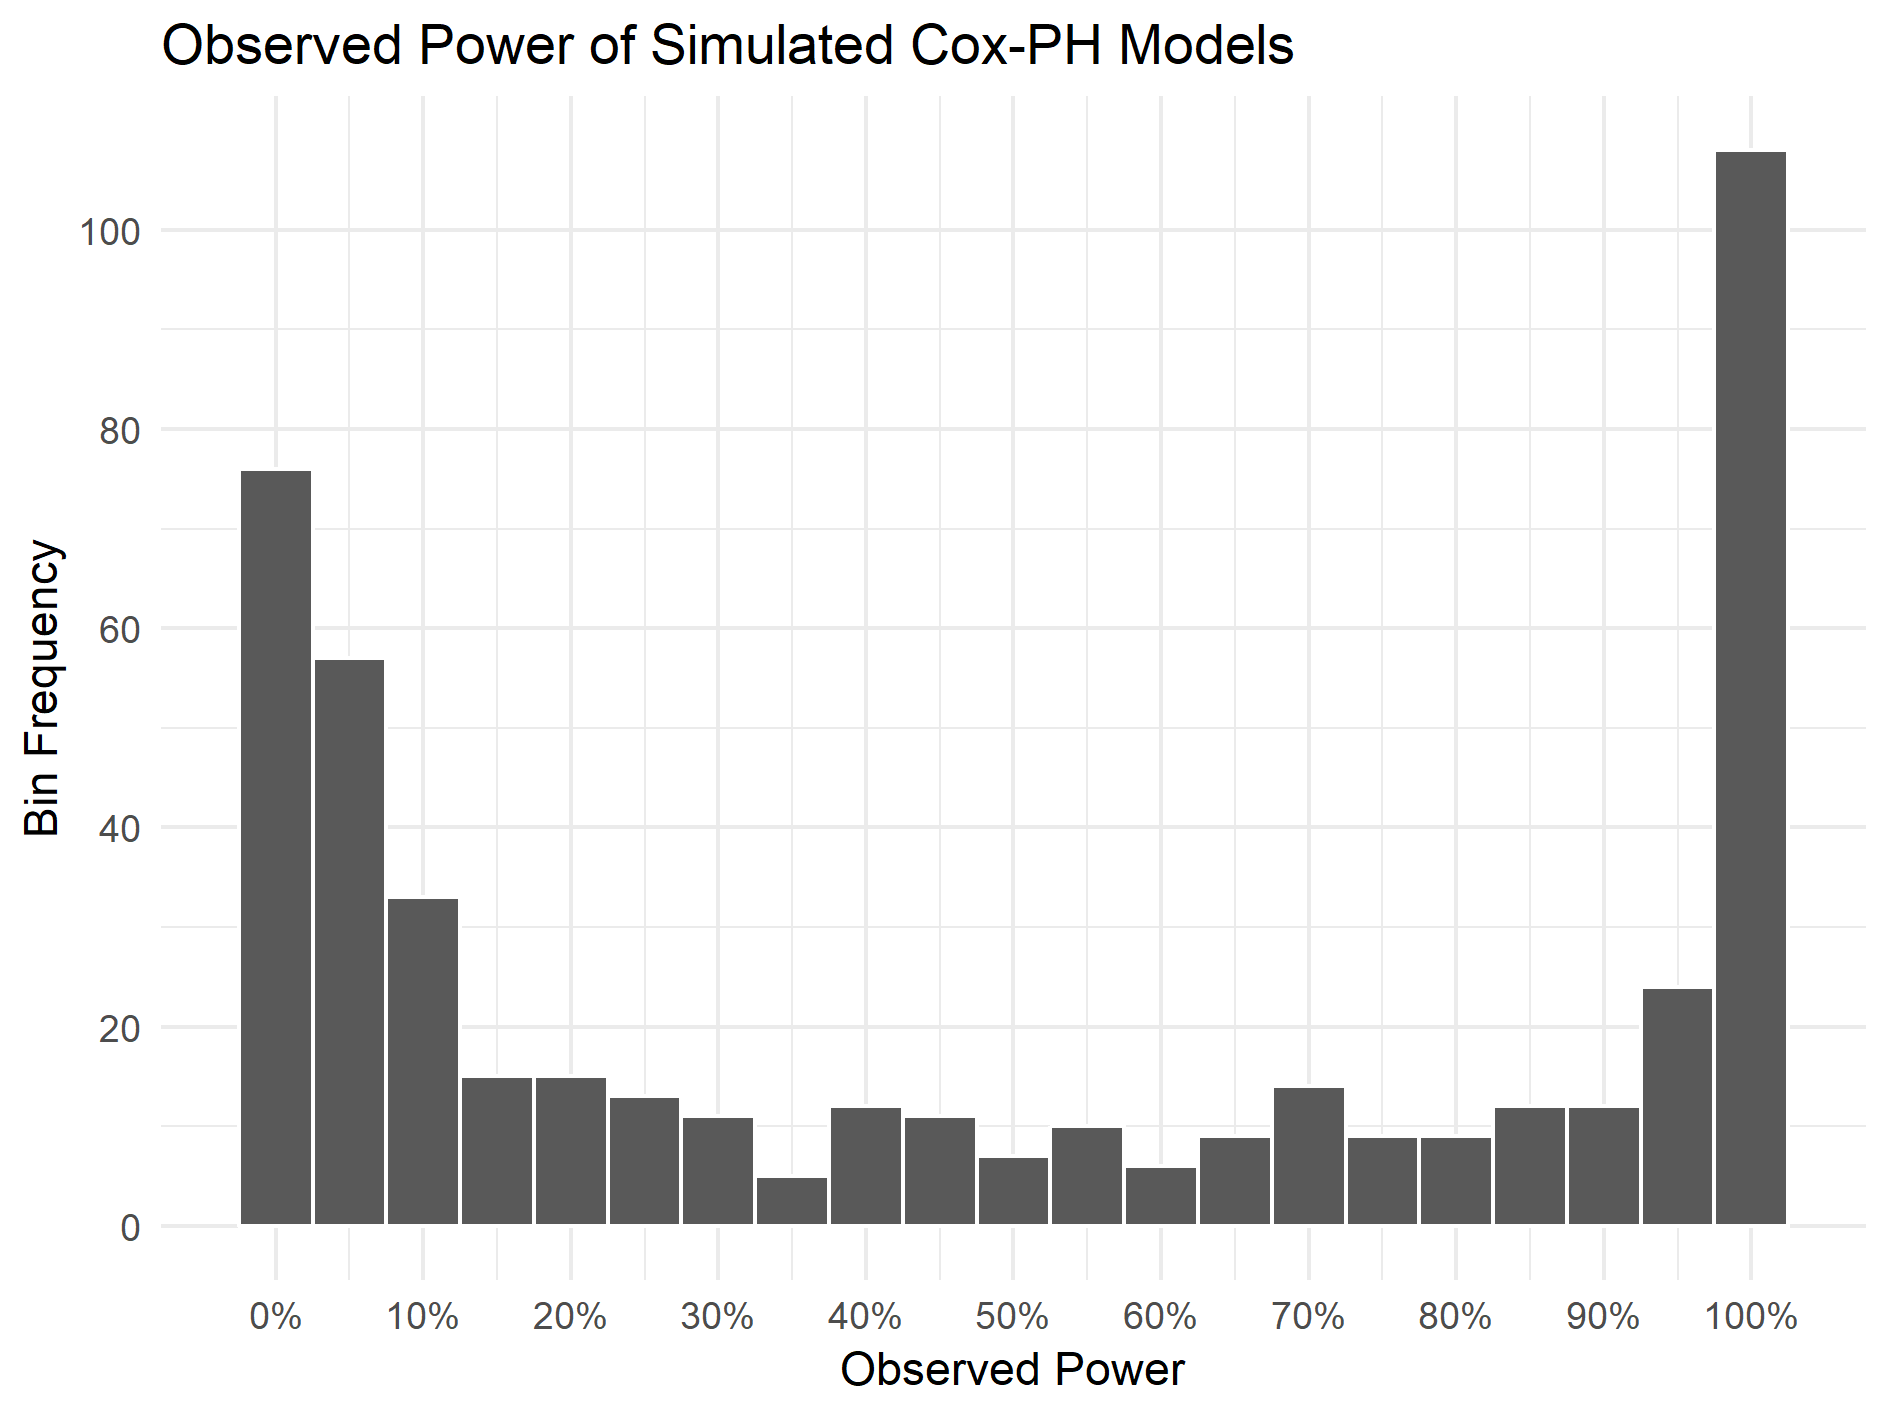
\includegraphics[width=\textwidth]{reports/figures/simulation-histogram.png}
% \end{figure}

% \begin{figure}
\caption[Effect of Baseline Hazard Rate on Power]{}
\label{fig:power-baseline-hazard}
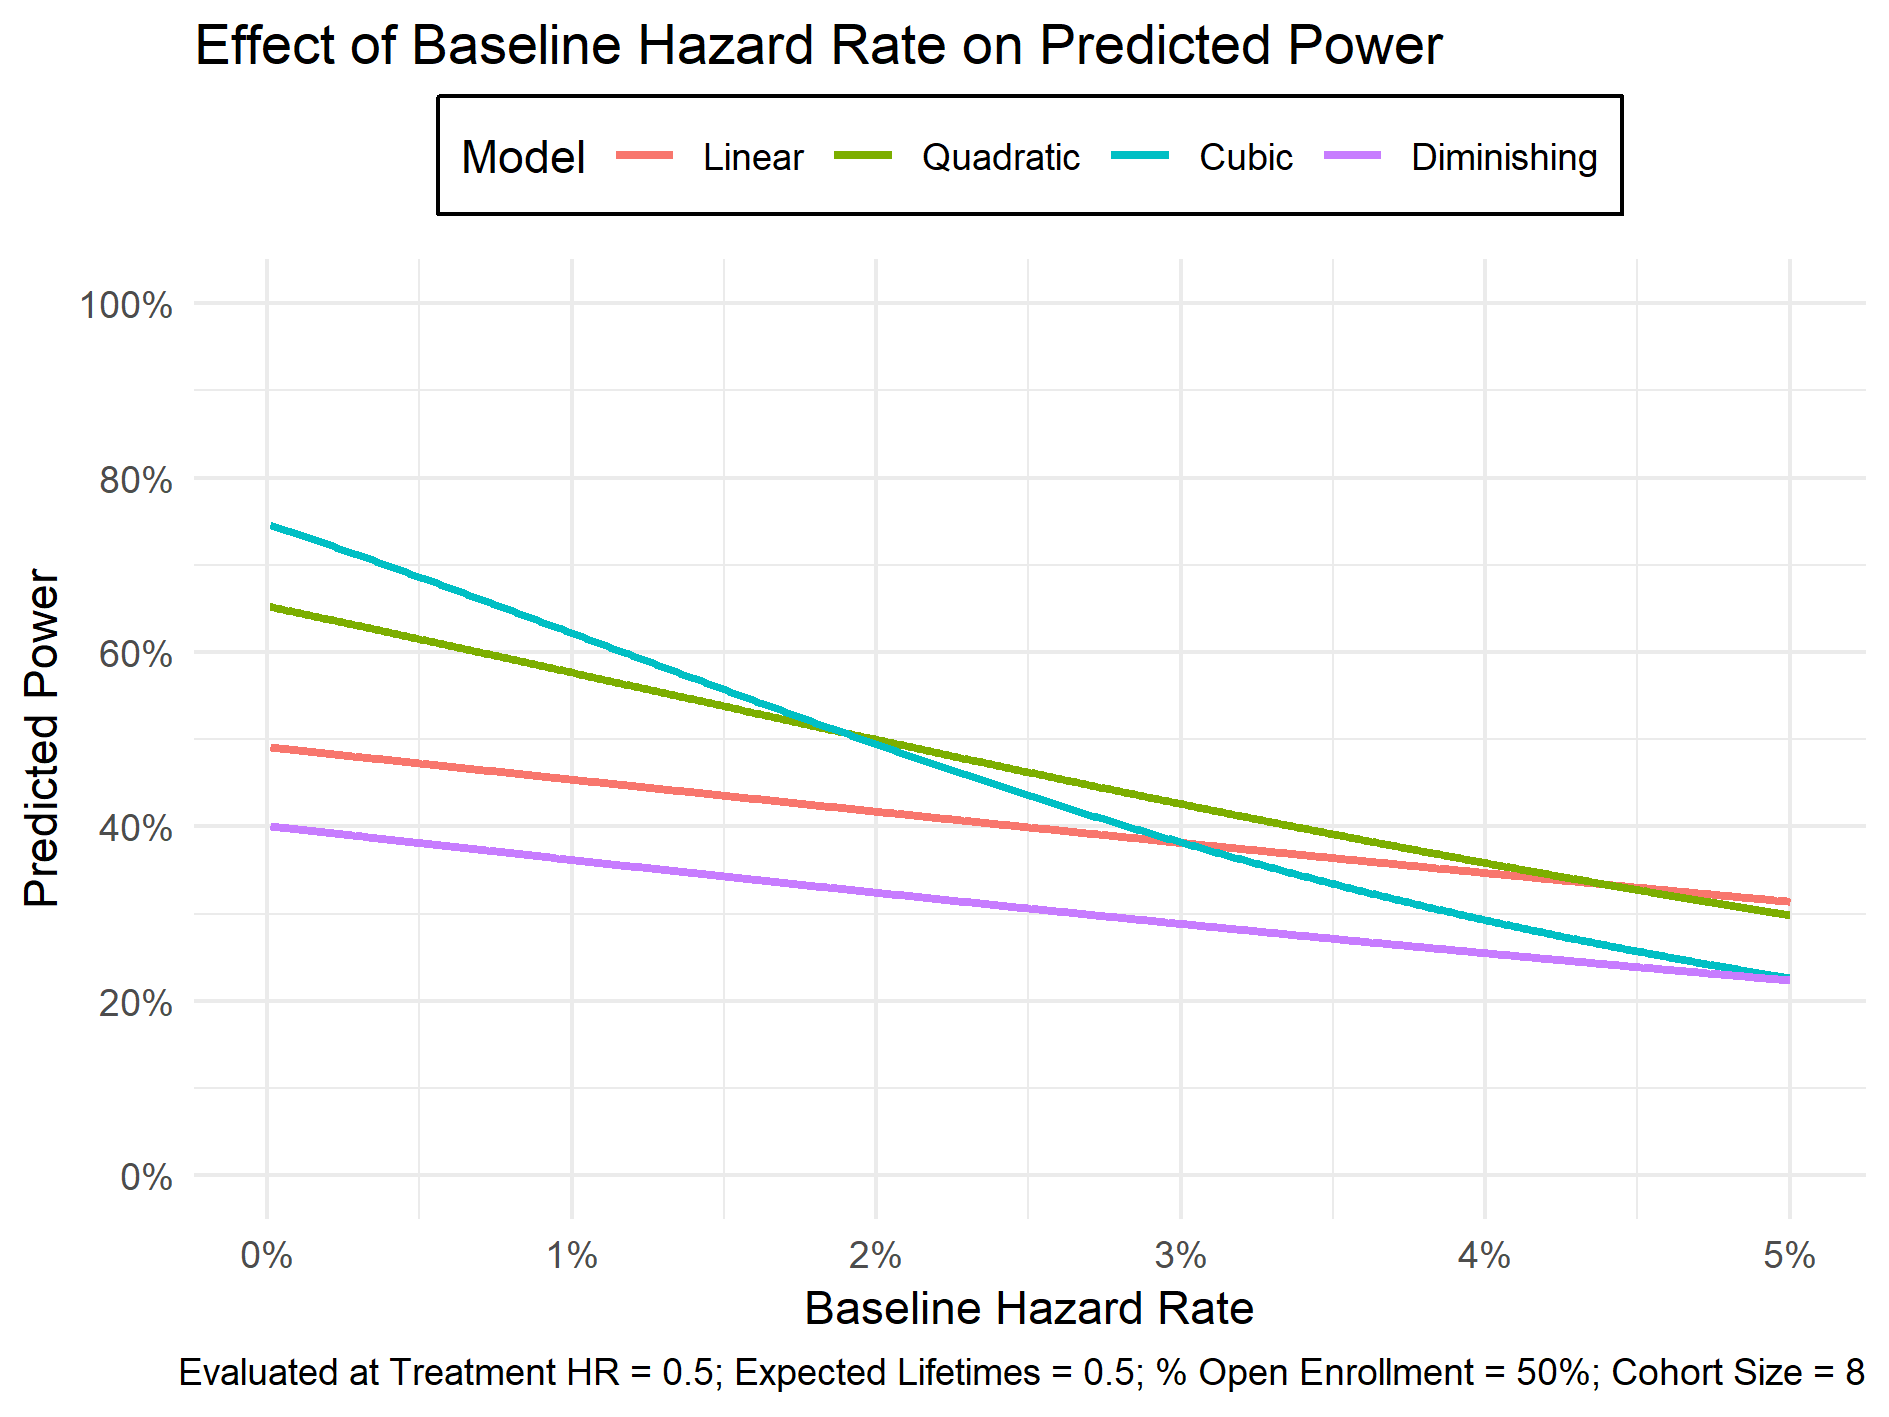
\includegraphics[width=\textwidth]{reports/figures/single-effects/power-baseline-hazard.png}
\end{figure}

\begin{figure}
\caption[Effect of Treatment Hazard Ratio on Power]{}
\label{fig:power-treatment-hr}
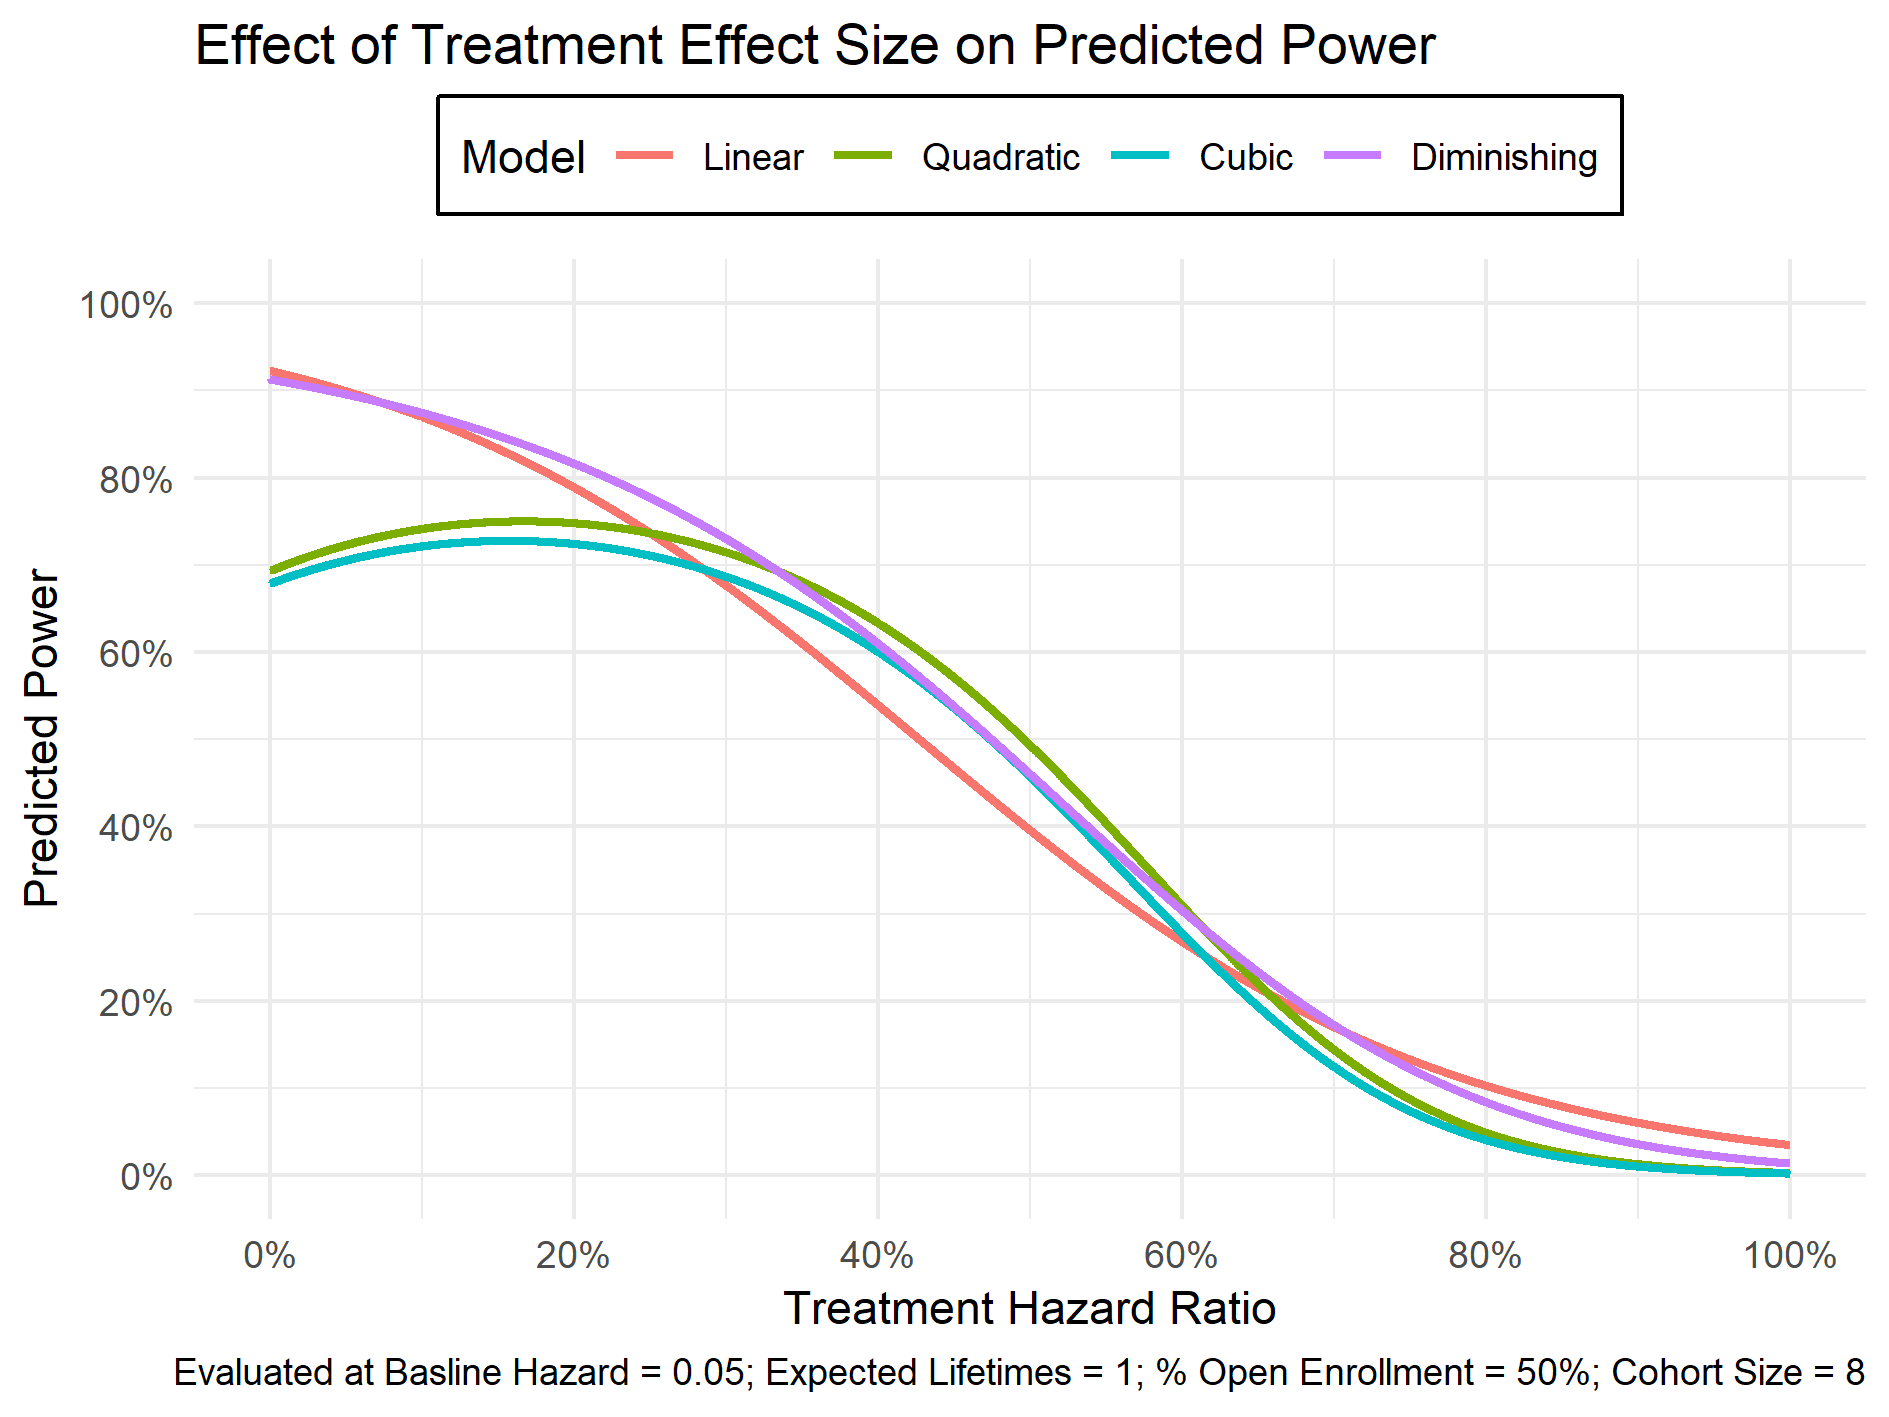
\includegraphics[width=\textwidth]{reports/figures/single-effects/power-treatment-hr.png}
% \end{figure}

% \begin{figure}
\caption[Effect of Cohort Size on Power]{}
\label{fig:power-cohort-size}
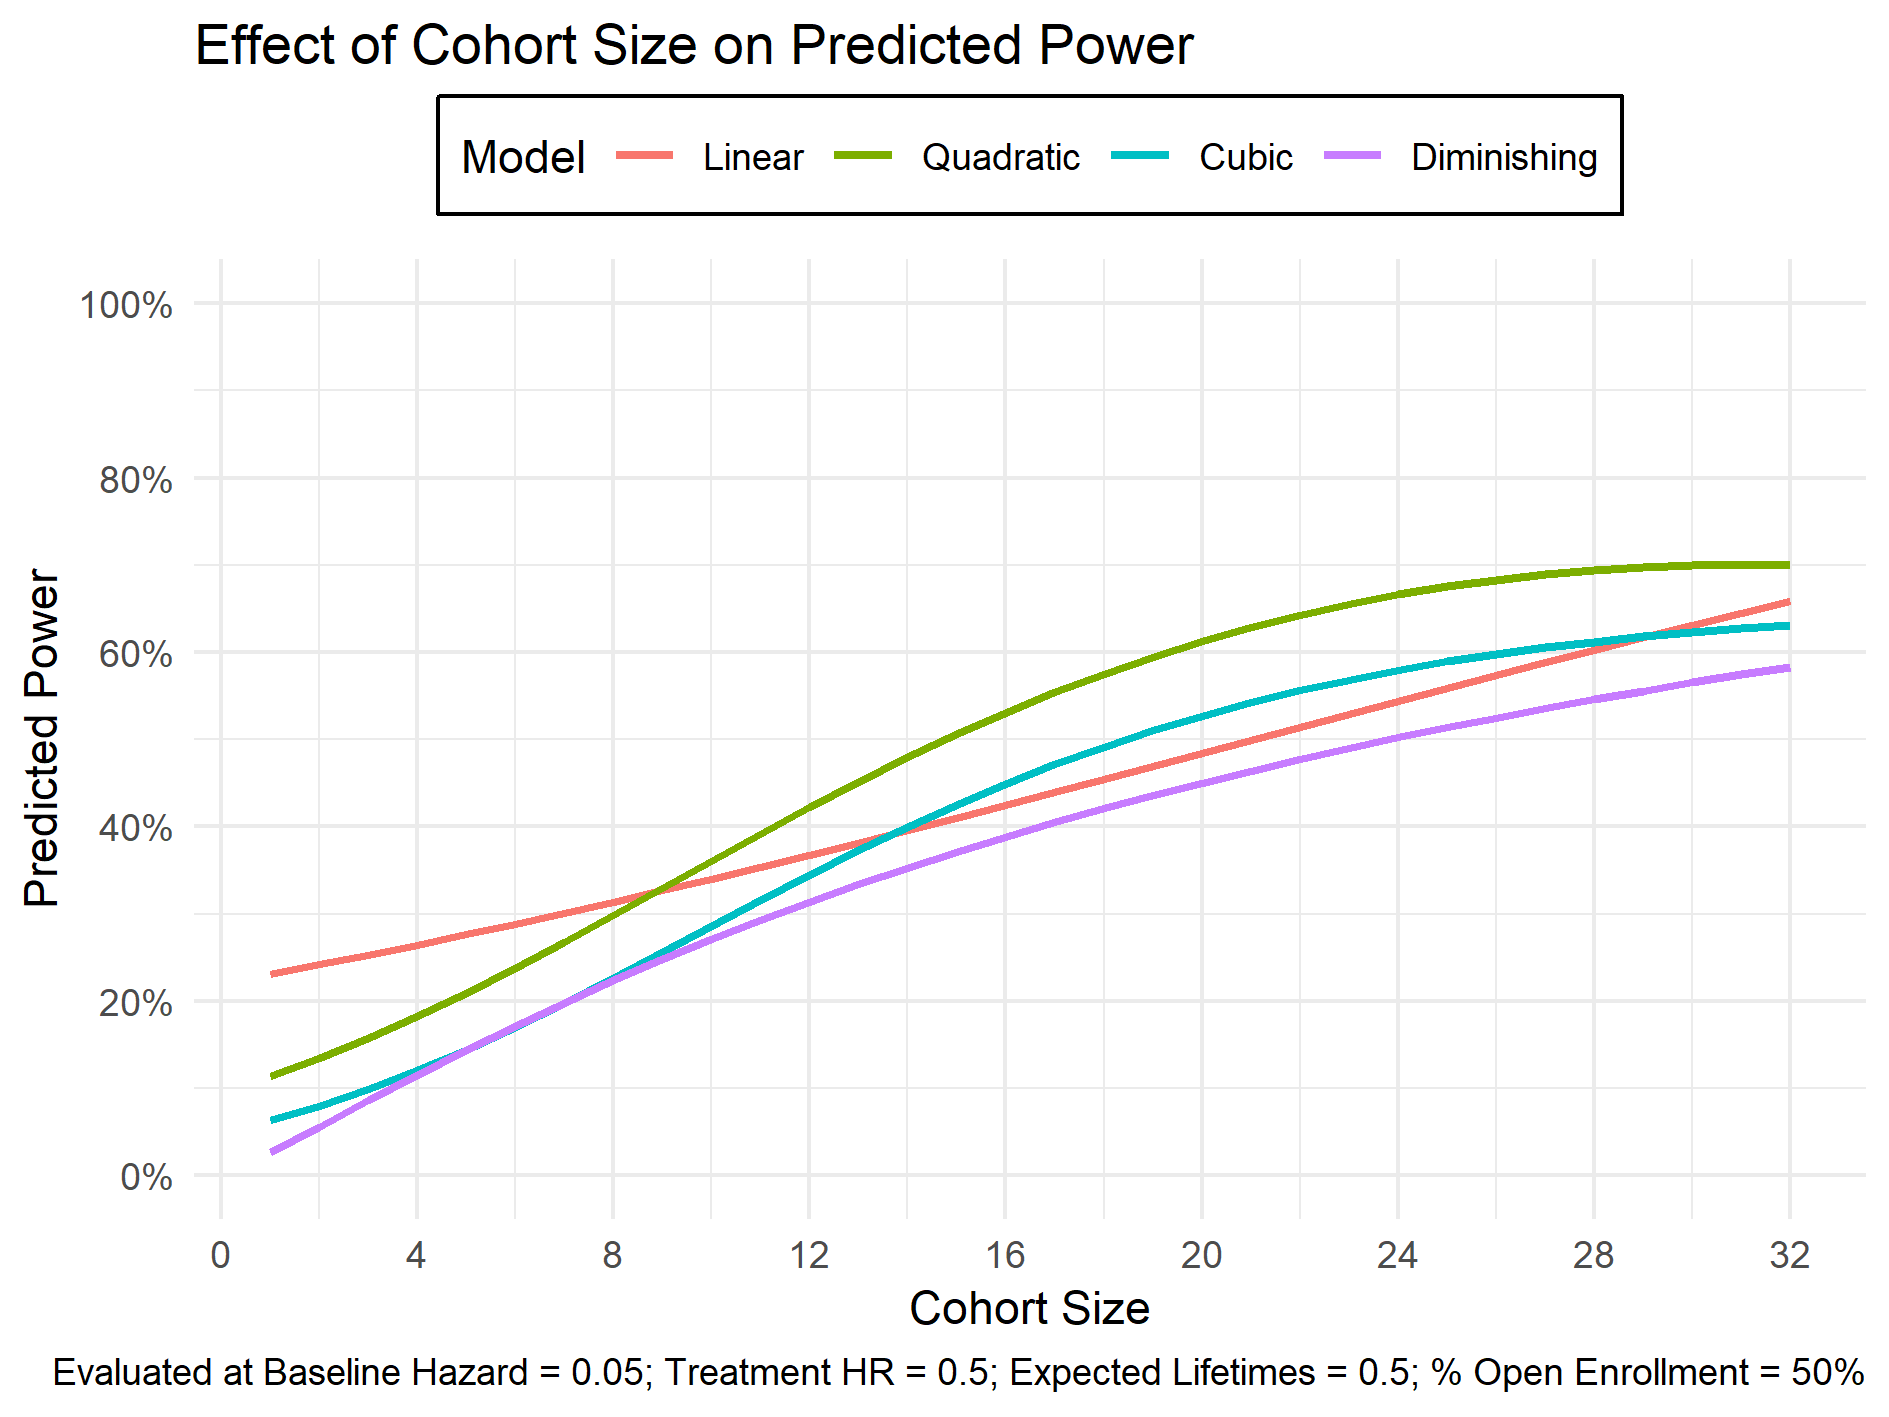
\includegraphics[width=\textwidth]{reports/figures/single-effects/power-cohort-size.png}
\end{figure}

\begin{figure}
\caption[Effect of Study Length on Power]{}
\label{fig:power-expected-lifetimes}
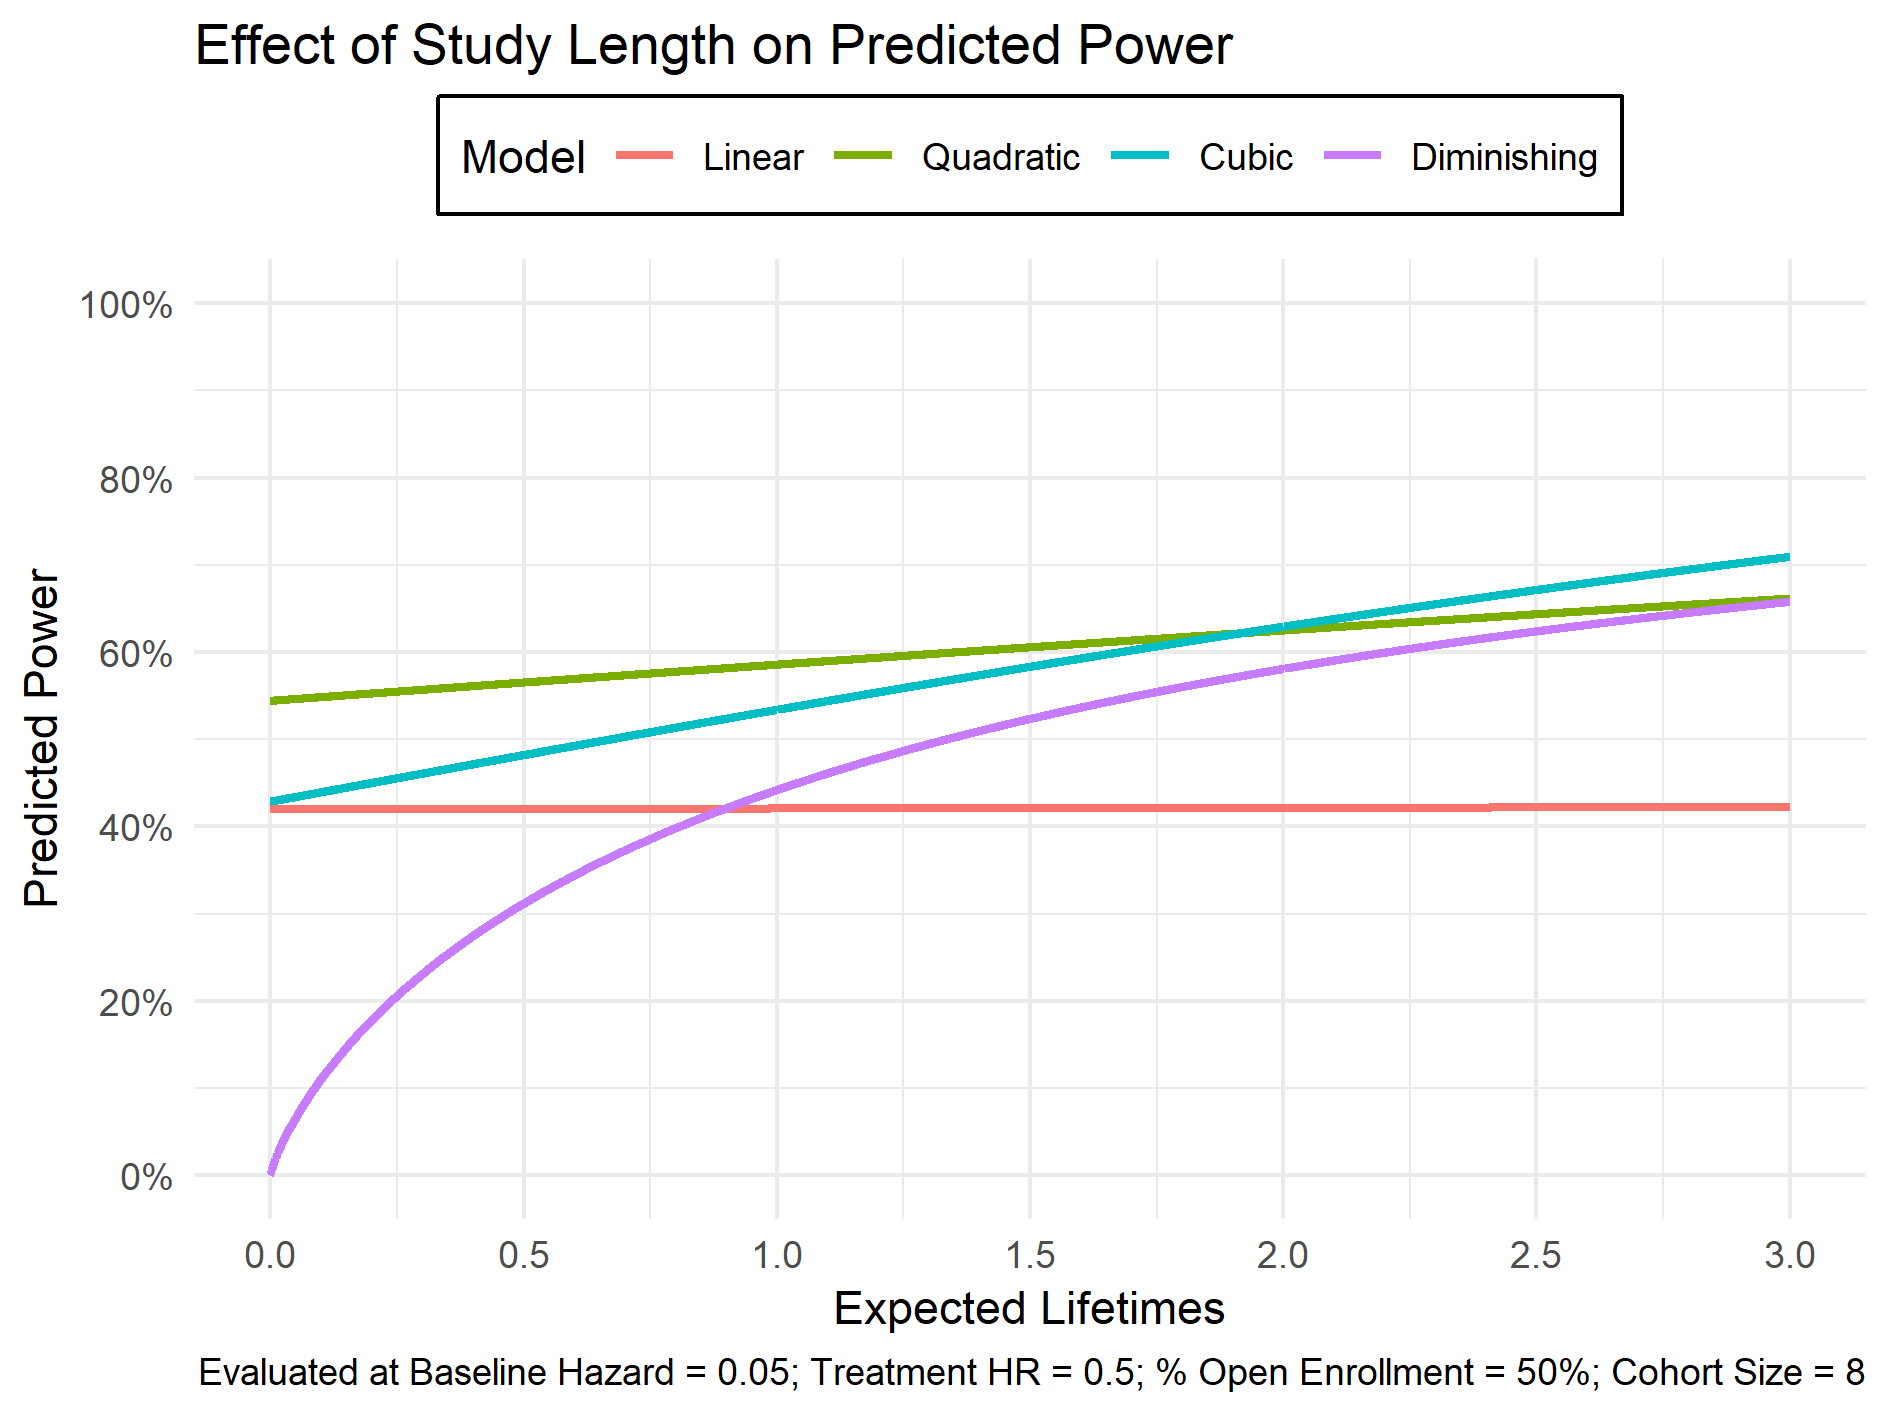
\includegraphics[width=\textwidth]{reports/figures/single-effects/power-expected-lifetimes.png}
% \end{figure}

% \begin{figure}
\caption[Effect of Study Length, Cohort Size on Power]{}
\label{fig:power-expected-lifetimes-cohort-size}
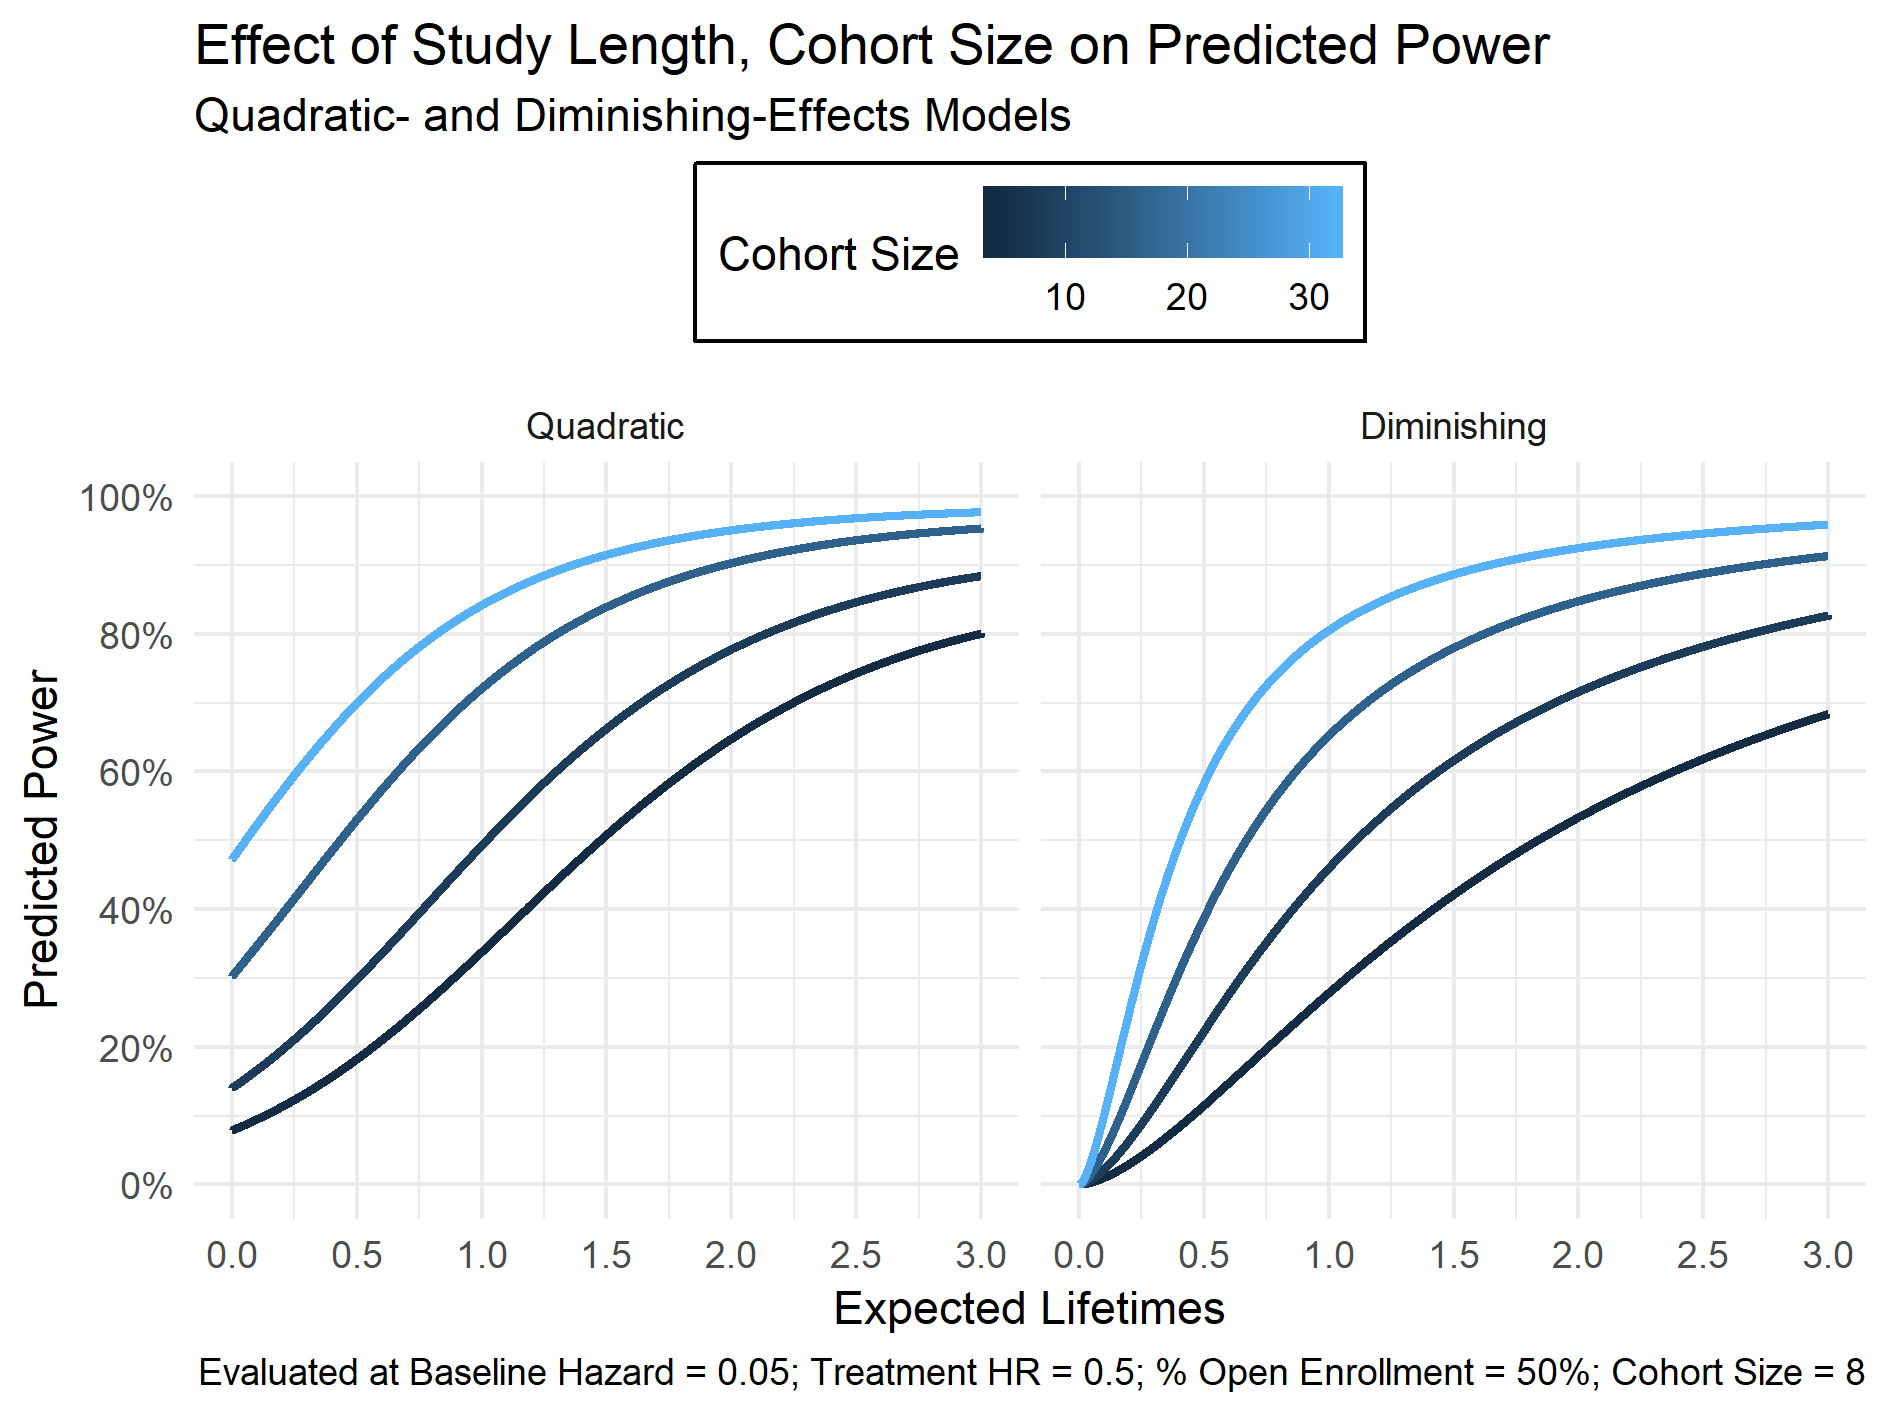
\includegraphics[width=\textwidth]{reports/figures/multiple-effects/power-expected-lifetimes-cohort-size.png}
\end{figure}


\begin{figure}
\caption[Effect of New Cohorts on Power]{}
\label{fig:power-pct-open-enrollment}
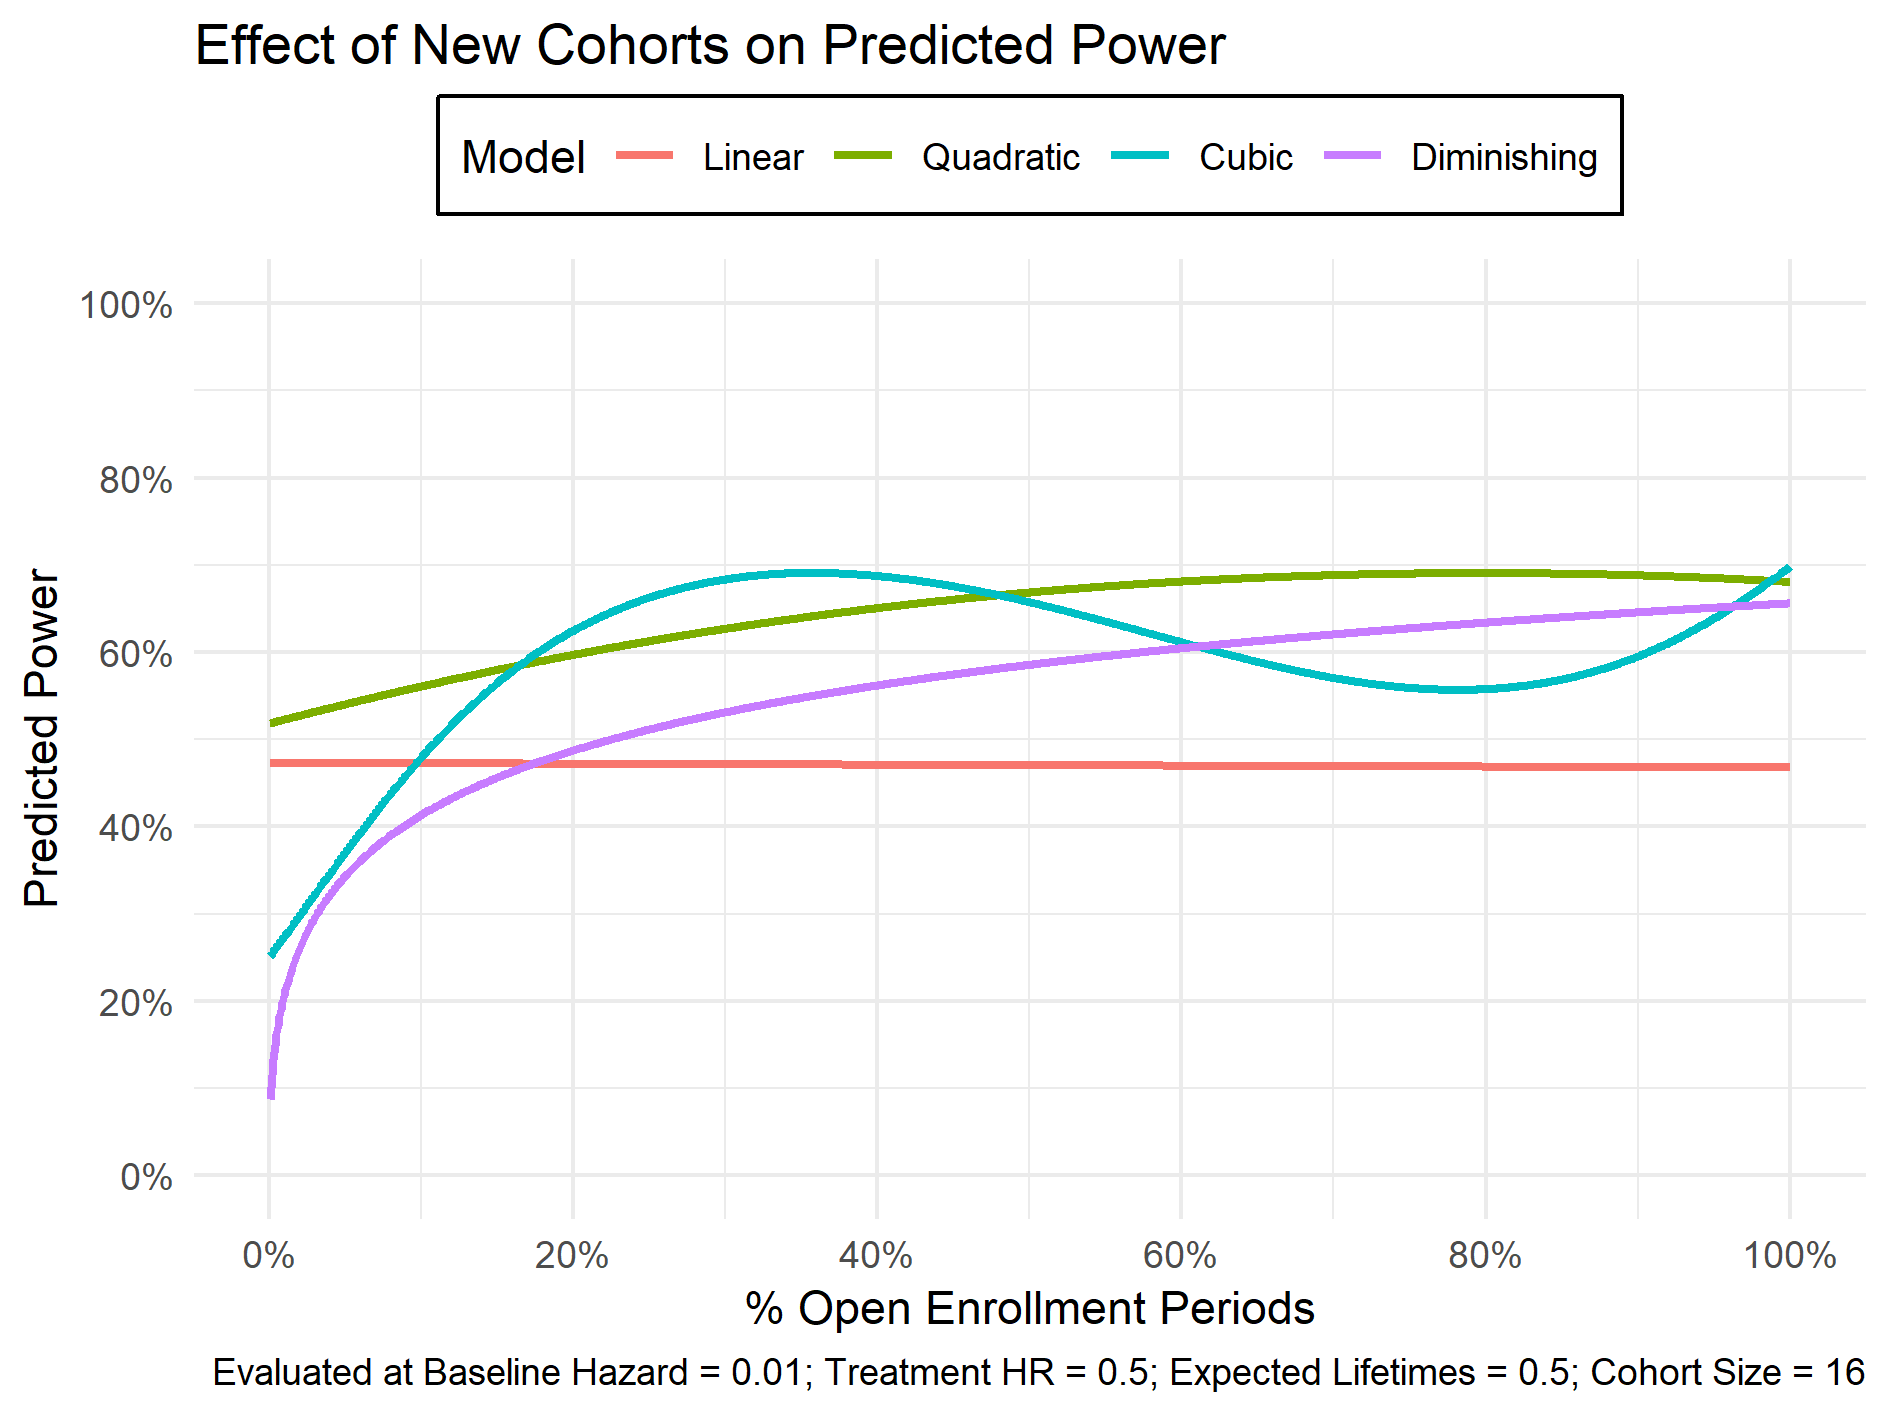
\includegraphics[width=\textwidth]{reports/figures/single-effects/power-pct-open-enrollment.png}
\end{figure}
